\section{Experiments with the baselines}
In this section, we will describe the experiments conducted using the baselines mentioned in Section \ref{sec:baselines}.
Since most of the relations from DBpedia are a sequence of words concatenated together as seen in Table \ref{tab:relations}. We first split the terms into individual tokens before we conduct the string similarity and the word embedding experiments.
\begin{table}[H]
    \centering
    \begin{tabular}{|c|c|}
     \hline
     \textbf{Relations from DBpedia} & \textbf{Split Relations} \\
    \hline
     foundedBy & founded By \\
    \hline
    associatedMusicalArtist & associated Musical Artist \\
    \hline
    foundingYear & founding Year \\
    \hline
    \end{tabular}
    \caption{Relations in DBpedia}
    \label{tab:relations}
\end{table}
\subsection{Experiment 1: String Similarity}
We first applied string matching techniques on the Free-Text knowledge graph and evaluated the results. Then, the similarity was calculated to test the resemblance between the tokenized keywords $kw_{i}$ and the list of relations in DBpedia $\mathcal{R}_{DB}$ (Section \ref{sec:relationsfromdbpedia}). 
We follow the steps below to obtain the results:
\begin{enumerate}
\item A question Q is first cleaned through the Text Preprocessing and Tokenization and Stop Word Removal modules used in the Section \ref{sec:TextCleaningPipeline} to get the keywords of the question.
\item  Q is not sent through the Lemmatization Module as the relation list from DBpedia is not lemmatized.
\item The similarity (\textit{Fuzzy-wuzzy ratio, Fuzzy-wuzzy partial ratio, Jaro metric, Jaro-Winkler metric}) of each keyword is computed with the list of relations in DBpedia $\mathcal{R}_{DB}$
\item relations are ranked based on the similarity score to get the Top k relations, k=5,10,15.
\end{enumerate}

Similar steps are followed for all the string matching techniques mentioned in Section \ref{sec:stringsimilarity}. Table \ref{tab:stringmatchingqald7} shows the results of the string matching techniques on QALD7.

Though string similarity is practical for words with spelling errors or plural forms of words, they do not capture the semantics of the keyword. String similarity techniques are successful for questions such as \textit{Who developed Slack?}, expected relation: \textit{dbo:developer}, where the keyword \textit{develop} is used for the search,
but \textbf{fail} to answer questions like \textit{Who is the host of the BBC Wildlife Specials?} where the expected relation: dbo:presenter cannot be matched with the keyword host.

\subsection{Experiment 2.a: Pre-trained Word Embeddings}
In this section, we detail the experiment carried out using the pre-trained word embeddings of word2vec to overcome the limitation of string similarity techniques. Cosine Similarity is calculated to test the resemblance between the tokenized keywords $kw_{i}$ and the list of relations in DBpedia $\mathcal{R}_{DB}$ that are matched to the embeddings in the vector space.
We follow the steps below to obtain the results:
\begin{enumerate}
\item Load the pre-trained word2vec model from gensim \footnote{\label{gensim}https://radimrehurek.com/gensim/}.
\item For each relation from $\mathcal{R}_{DB}$,
\begin{enumerate}
    \item Split the relation to tokens as some relations in Dbpedia are concatenated strings of tokens.
    \item Map each word in the relation to its word vector if it is present in the word2vec model vocabulary. If the word vector is not present the word is not considered. 
\end{enumerate}
\item A question Q, is first cleaned through the Text Preprocessing, and Tokenization and Stop Word Removal modules used in the Section \ref{sec:TextCleaningPipeline} to get the keywords of the question.
\item  Q is not sent through the Lemmatization Module as the relation list from DBpedia is not lemmatized.
\item Each keyword in the question is mapped to its word vector in the word2vec model if it is present in the word2vec model vocabulary.
\item The cosine similarity of each vectorized  keyword is computed with the vectorized list of relations $\mathcal{R}_{DB}$
\item Relations are ranked based on the similarity score to get the Top k relations, k=5,10,15.
\end{enumerate}
Table \ref{tab:stringmatchingqald7} shows the results for pre-trained word embeddings on QALD-7.

The pre-trained word embedding approach had the constraint of out of vocabulary words. Some of the tokens mentioned in the relations were not found in the word2vec vocabulary.

\subsection{Experiment 2.b: Custom Word Embeddings}
In this section, we discuss the experiment carried out using the custom word embeddings created from $\mathcal{R}_{DB}$. We follow the steps below to obtain the results:
\begin{enumerate}
\item For each relation in $\mathcal{R}_{DB}$, split the concatenated relation to tokens.
\item Create a vector model using the split list of relations obtained. We use the Doc2Vec\footnote{https://radimrehurek.com/gensim/models/doc2vec.html} model from gensim.
\item A question Q is first cleaned through the Text Preprocessing, Tokenization and Stop Word Removal modules to get the keywords of the question.
\item  Q is not sent through the Lemmatization Module as the relation list from DBpedia is not lemmatized.
\item The vector of each keyword in the question is inferred from the Doc2vec model.
\item The cosine similarity is computed between a simple mean of the projection weight vectors of each vectorized keyword and the vectors for each word in the model.
\item Relations are ranked based on the similarity score to get the Top k relations, k=5,10,15.
\end{enumerate}
Table \ref{tab:stringmatchingqald7} shows the results for custom word embeddings on QALD-7.

\subsection{Experiment 3: TF-IDF}
We use the TF-IDF technique on the Free-text KG as an improvised baseline from string matching and word embeddings. For the TF-IDF method we use the relation files that have the tokenized subject-object sentences from Section \ref{usingfreetextkg}. Given below are the steps to compute TF-IDF:
\begin{enumerate}
    \item Count the number of relation files in \textbf{FTKG\_fileList} and assign an id to each file.
    \item Pre-process the contents of each file by passing through the Text Cleaning Pipeline in Section \ref{sec:TextCleaningPipeline}.
    \item Iterate through the files and calculate the Term Frequency and the Document Frequency of the words.
    \item Calculate the TF-IDF for the contents of the file.
    \item A question Q is first cleaned the Text Cleaning Pipeline to get the keywords of the question. 
    \item Matching score is calculated to evaluate how similar the words in the document are with respect to the keywords of the question. The score is obtained by adding TF-IDF values of the tokenized keywords that are in the question for every document.
    \item The relations are ranked based on the similarity score to get the Top k relations, k=5,10,15.
\end{enumerate}
Table \ref{tab:stringmatchingqald7} shows the results for TF-IDF method on QALD-7.

\begin{table}[H]
    \centering
    \begin{tabular}{|c|c|c|c|}
     \hline
     \textbf{String Matching} & \textbf{Hits@5} & \textbf{Hits@10} & \textbf{Hits@15}  \\
    \hline
     FuzzyWuzzy ratio & 0.28 & 0.35	& 0.37 \\
    \hline
    FuzzyWuzzy partial ratio & 0.06 & 0.17 & 0.24 \\
    \hline
        Jaro  & 0.30 & 0.37	& 0.38 \\
    \hline
        Jaro-Winkler & 0.31 & 0.39 &0.40 \\
    \hline
        Doc2Vec & 0.16 & 0.22 & 0.23 \\
    \hline
        TFIDF & 0.11 & 0.23 & 0.27 \\
    \hline
        \textbf{ReMLOFT} & \textbf{0.61} & \textbf{0.68} & \textbf{0.69} \\
    \hline
    \end{tabular}
    \caption{String Matching Results on QALD-7}
    \label{tab:stringmatchingqald7}
\end{table}

\section{Results}
In this section, we discuss the findings from the experiments over our datasets and baselines.
We first evaluated the Hits@k (k=5,10,15) for the First intersection candidate relations  $Candidate\_List_{First\cap}$ (Refer Section. \ref{sec:candidatelist}). Figure. \ref{fig:firstHits} shows that the Hits@k value for the datasets increases significantly when k is increased. This is due to the fact that, as the complexity of the question increases, the number of expected relations to build a SPARQL query increases. We notice a convincing increase when we evaluate the Hits@k (k=5,10,15) for the Final intersection candidate relations  $Candidate\_List_{Final\cap}$ (Refer Section. \ref{sec:candidatelist}). The two-hop relations are captured in the final intersection candidates for questions having answers two hops away. 
It is clear from Table \ref{tab:stringmatchingqald7} that ReMLOFT has a higher results as compared to all other baselines when implemented on QALD-7.

\begin{figure}[p]
    \centering
    \begin{minipage}{0.7\textwidth}
   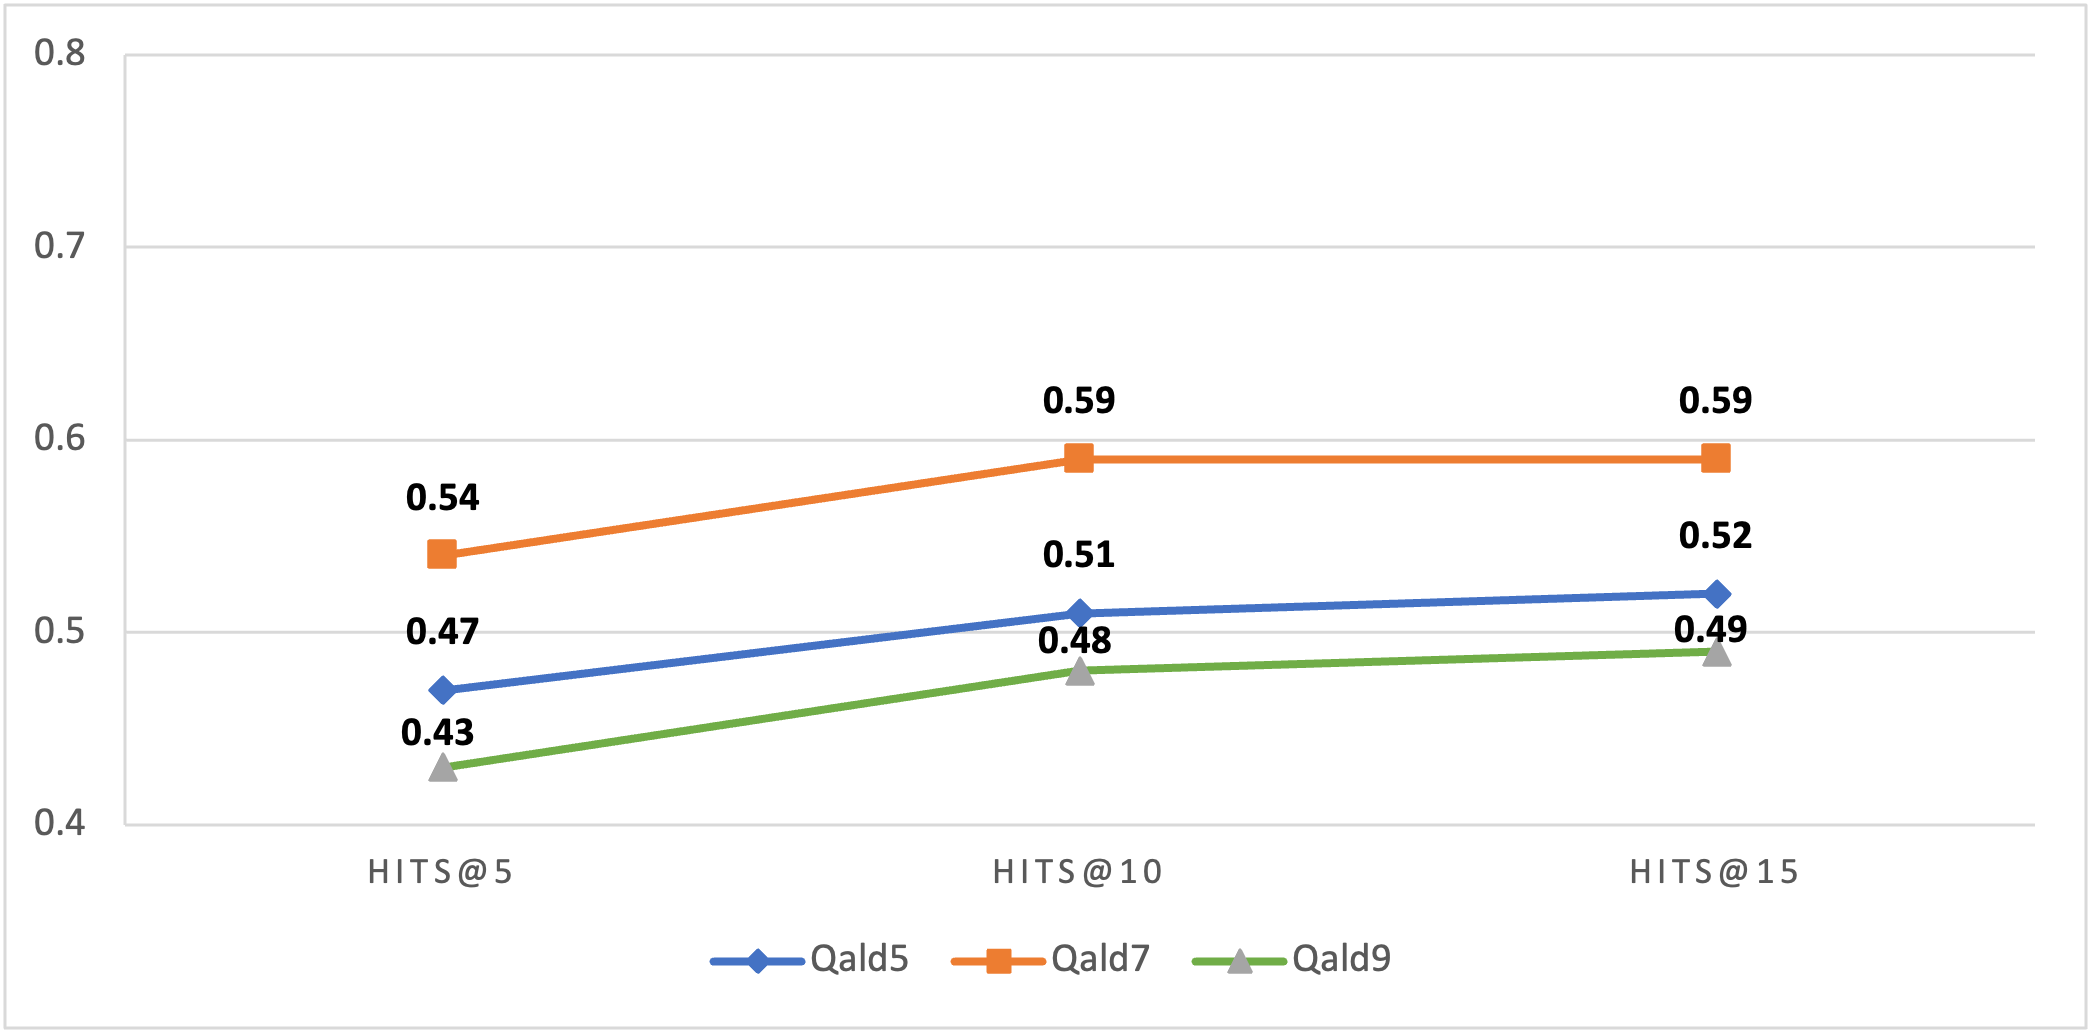
\includegraphics[width=\textwidth]{chapters/figures/firstHits.png}
    \caption{Hits@k for the First Intersection}
    \label{fig:firstHits}
     \end{minipage}
         \begin{minipage}{0.7\textwidth}
   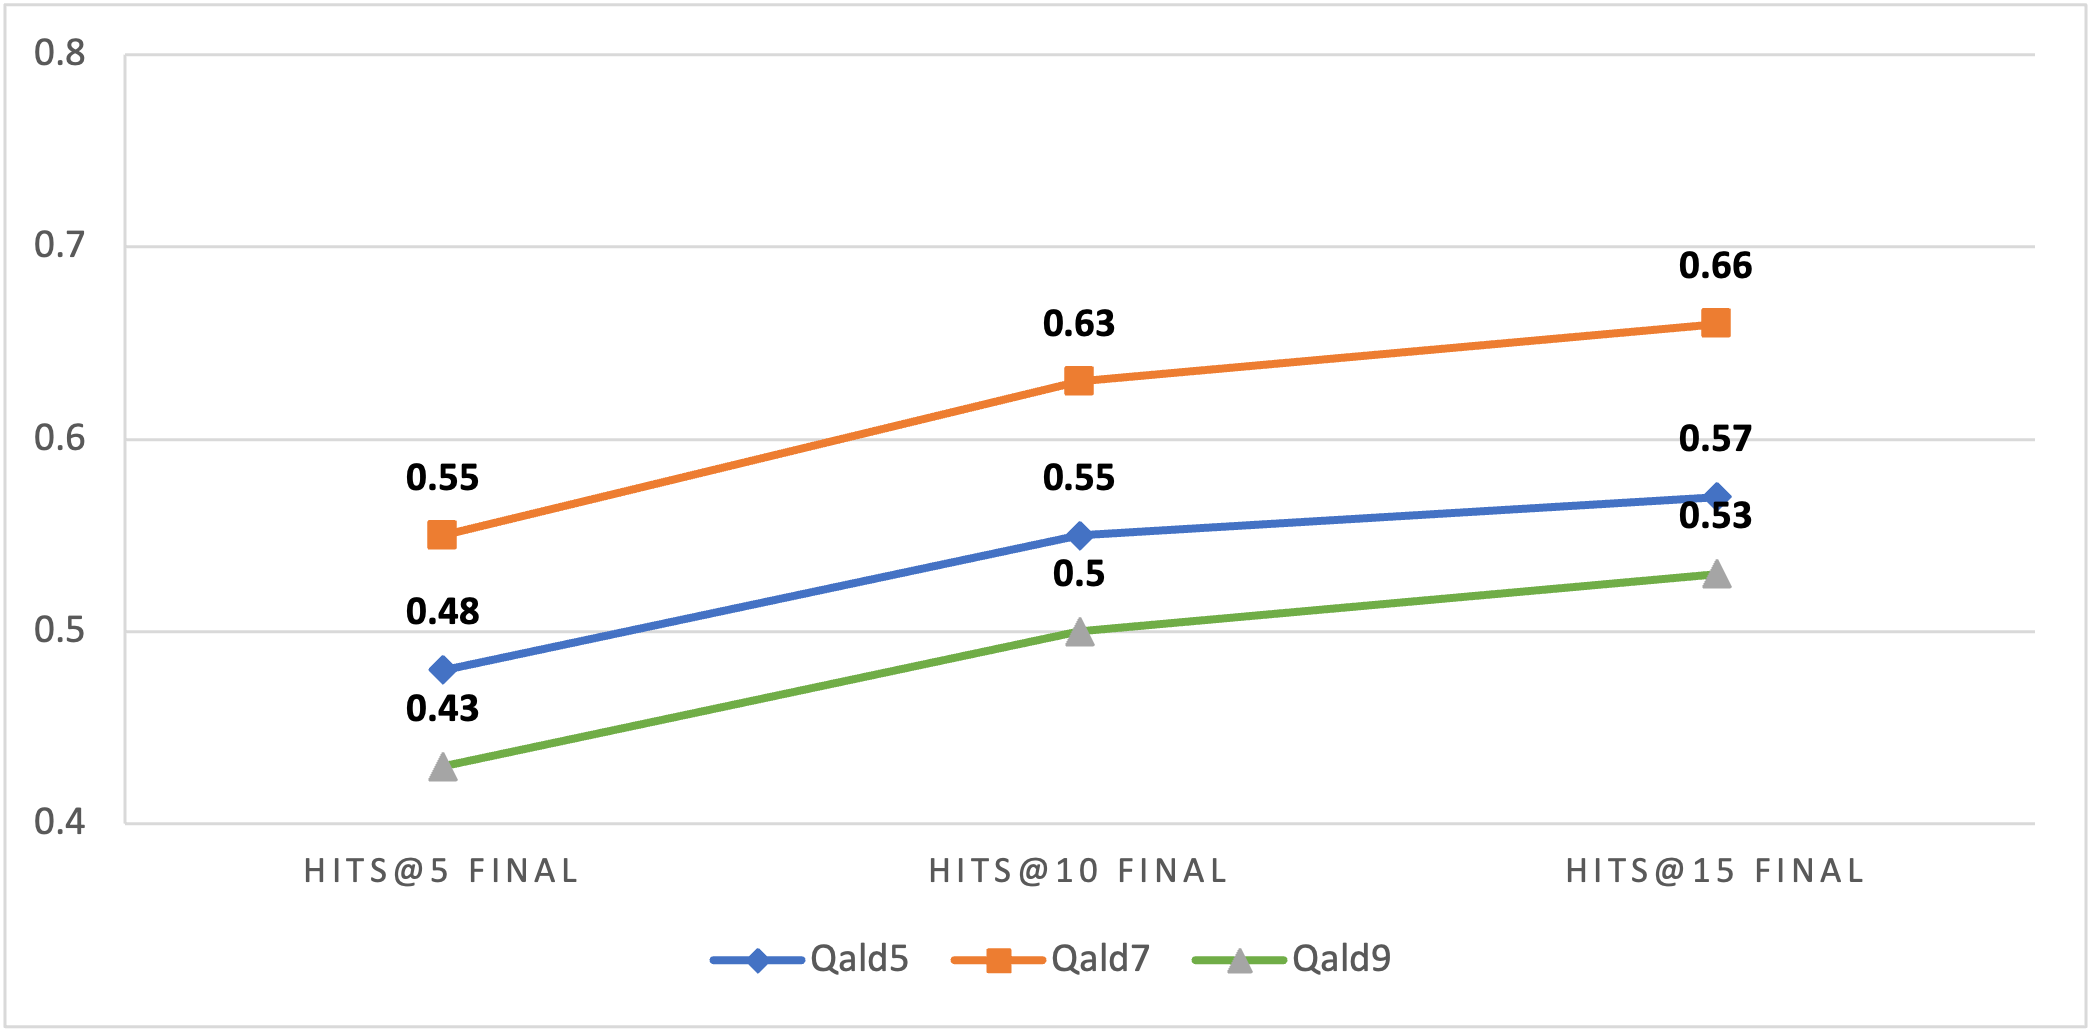
\includegraphics[width=\textwidth]{chapters/figures/finalHits.png}
    \caption{Hits@k for the Final Intersection}
    \label{fig:finalHits}
     \end{minipage}
         \begin{minipage}{0.7\textwidth}
    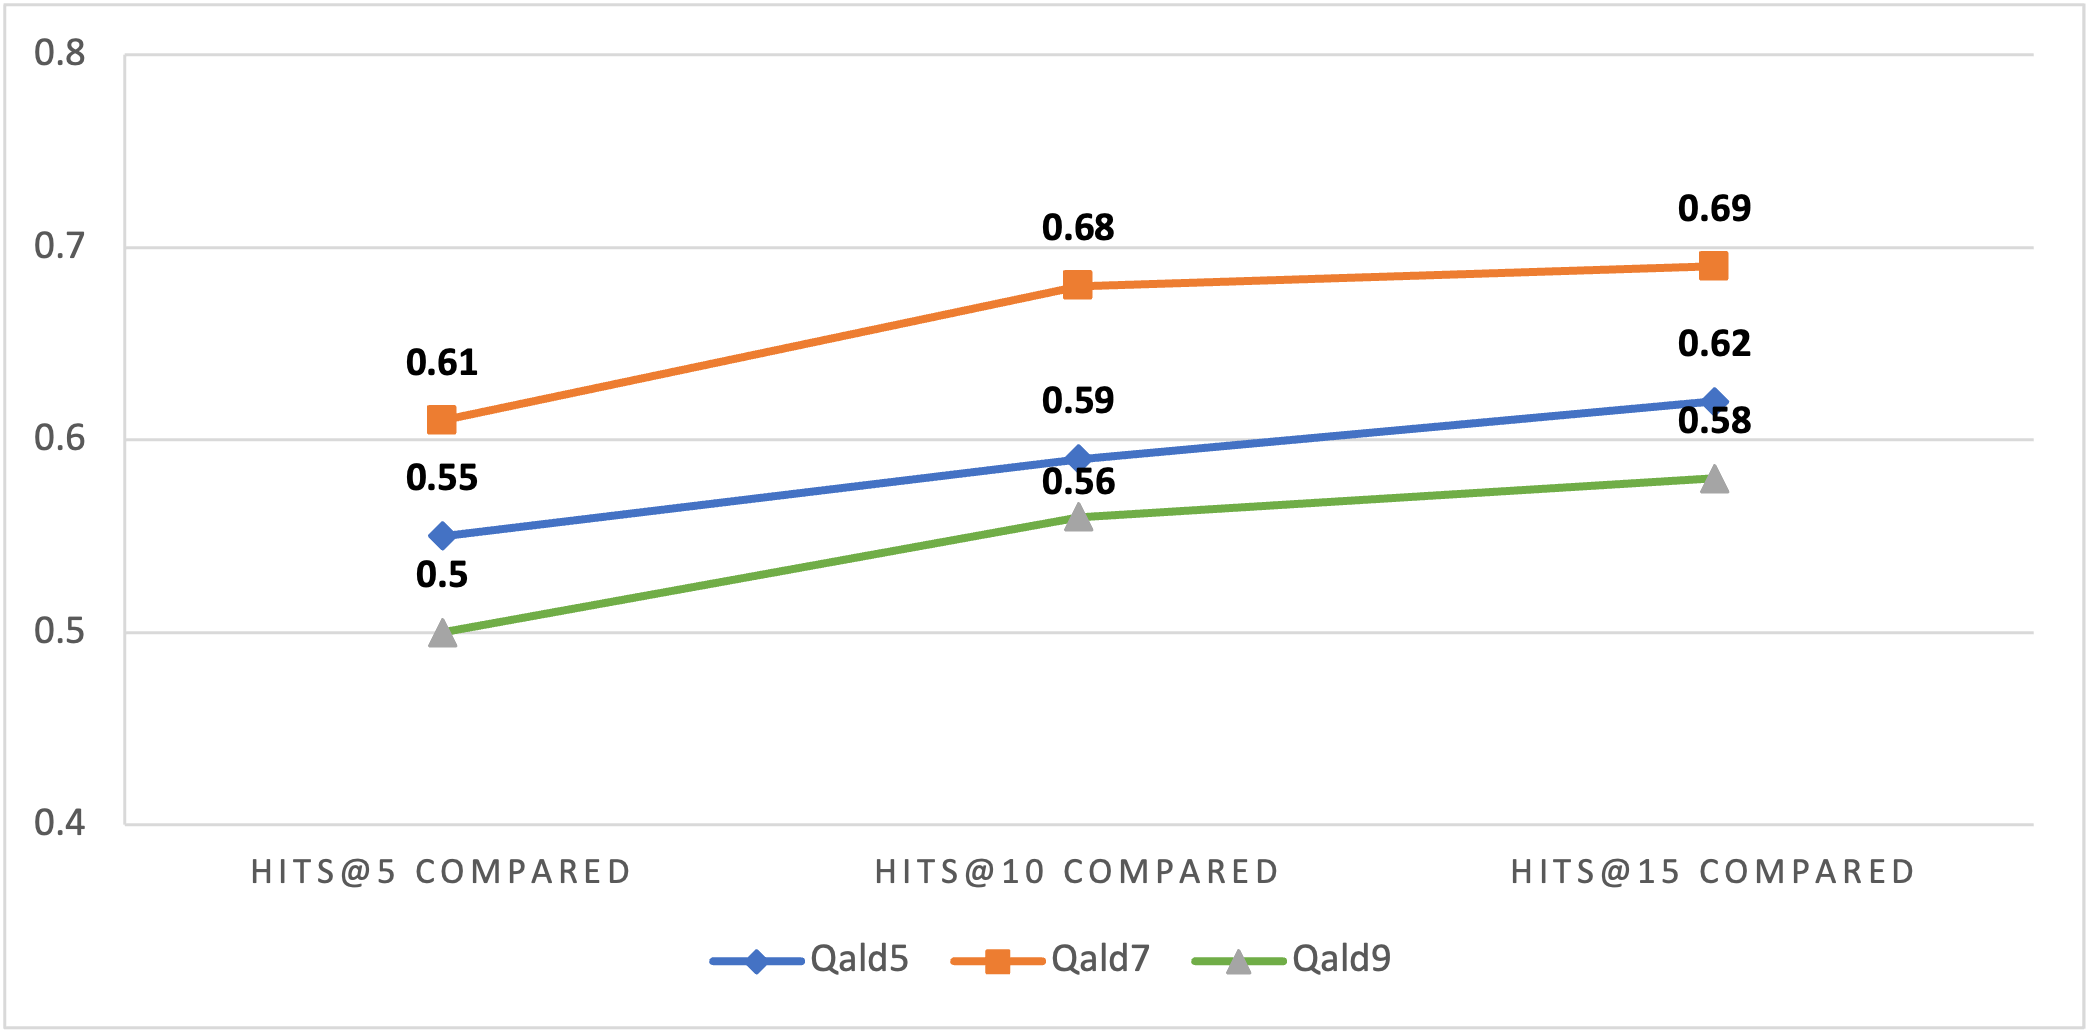
\includegraphics[width=\textwidth]{chapters/figures/ComparedHits.png}
        \caption{Hits@k for the Improved Result}
        \label{fig:ComparedHits}
    \end{minipage}
\end{figure}

The coverage results of ReMLOFT for the QALD datasets are shown in Table \ref{tab:relationcoverage}. ReMLOFT performs exceptionally for complex questions with more than one relation and has adequate coverage for simple questions. The best scores are highlighted in Table \ref{tab:relationcoverage}. We see that ReMLOFT performs well for questions with two relations across all the datasets with nearly \textbf{80\%} coverage. 
\begin{table}[H]
    \centering
    \begin{tabular}{|c|c|c|c|c|}
     \hline
     \textbf{No of Relations} & \textbf{QALD-5} & \textbf{QALD-7} & \textbf{QALD-9}  \\
    \hline
     1 Relation & 0.65 & 0.71	& 0.61 \\
    \hline
    2 Relations & \textbf{0.83} & \textbf{0.83} & \textbf{0.80} \\
    \hline
    3 Relations & 0.63 & \textbf{1}	& \textbf{0.83} \\
    \hline
    4 Relations & \textbf{1} & - & 0 \\
    \hline
        Total Coverage & 0.69 & 0.74 & 0.65 \\
            \hline
    \end{tabular}
    \caption{ReMLOFT Coverage(*100) for Questions based on Number of relations}
    \label{tab:relationcoverage}
\end{table}

The accuracy of ReMLOFT varies based on the number of questions in the dataset. ReMLOFT returns 163 relations from a total of 262 relations for QALD-5, 142 relations from a total of 209 relations for QALD-7 and 259 relations from a total of 441 relations for QALD-9. Figure \ref{fig:graphacc} shows that ReMLOFT represents a vast improvement in accuracy when compared to our baselines.

\begin{figure}
    \centering
   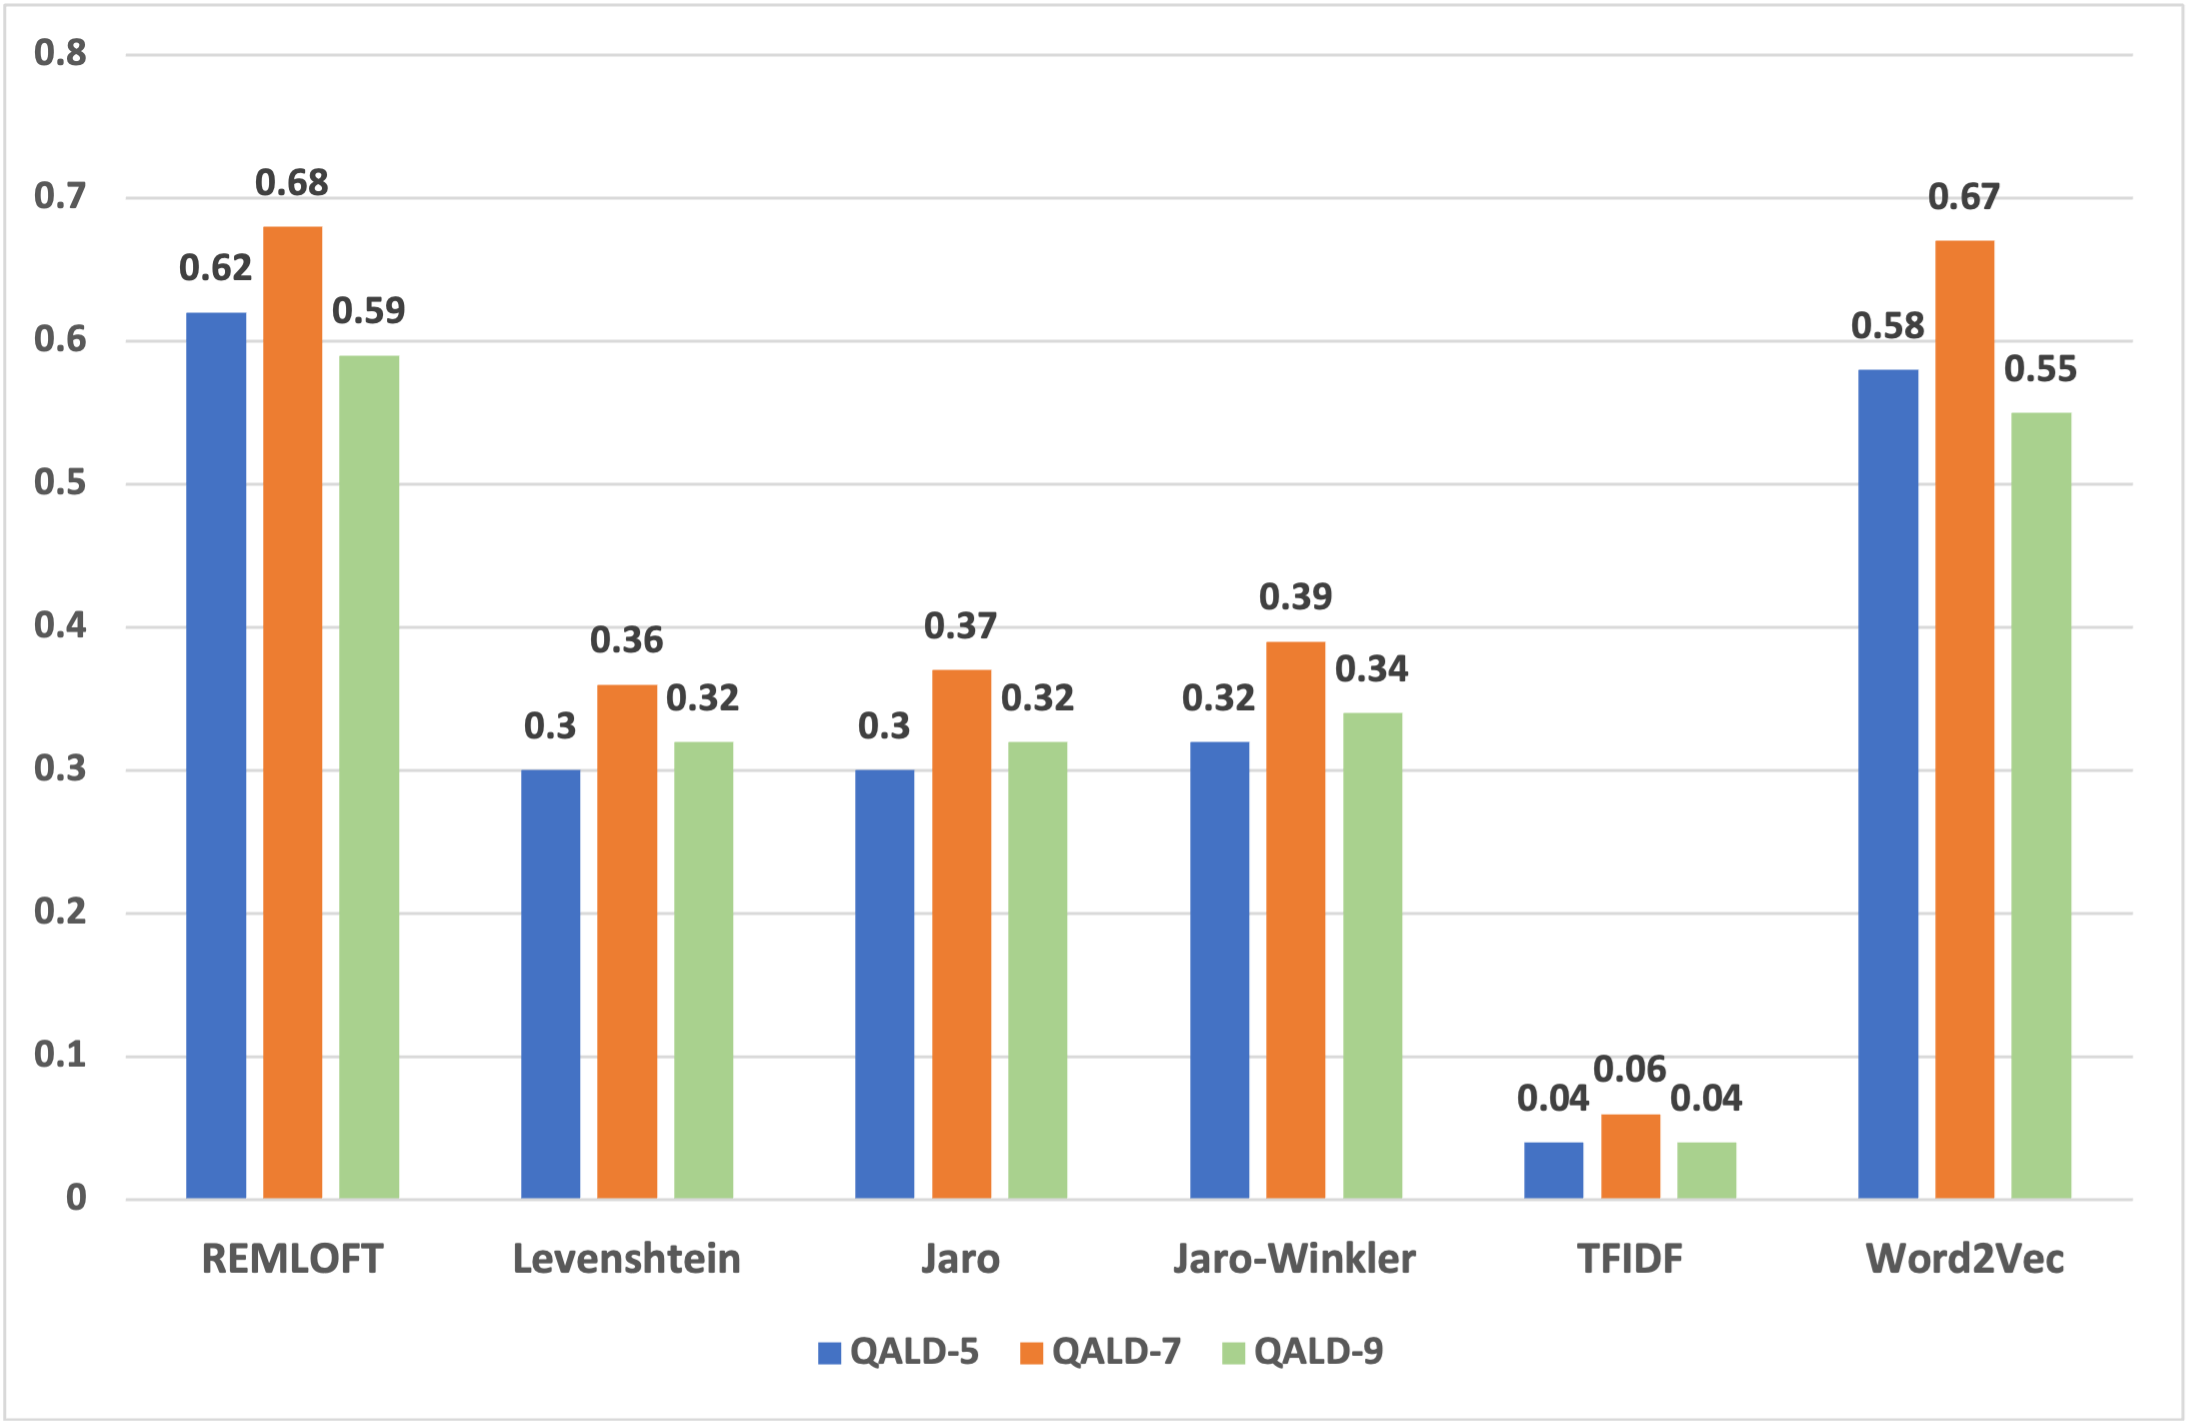
\includegraphics[width=10cm, height=5cm]{chapters/figures/Accuracy.png}
    \caption{Accuracy(*100) of ReMLOFT vs other baselines}
    \label{fig:graphacc}
\end{figure}

\begin{table}[H]
    \centering
    \begin{tabular}{|c|c|c|}
     \hline
     \textbf{Datsets} & \textbf{Accuracy} \\
    \hline
     QALD-5 & 0.62 \\
    \hline
    QALD-7 & 0.68 \\
    \hline
        QALD-9 & 0.59 \\
    \hline
    \end{tabular}
    \caption{Accuracy(*100) of ReMLOFT}
    \label{tab:accuracy}
\end{table}




% \left\{\begin{matrix}
% \left| a \right| & if \ \left| b \right|=0, \\
% \left| b \right| & if \ \left| a \right|=0, \\
% 1+min{lev}\_{a,b}(i-1,j) + 1  & if \ a[0]=b[0], \\
% {lev}\_{a,b}(i,j-1) + 1 & \\
% {lev}\_{a,b}(i-1,j-1) + 1  &\\
% \end{matrix}\right.

\textbf{Questions with rdf:type.} Questions whose SPARQL query requires the rdf:type to be retrieved doesn't work well with our approach. Consider an example question, \textbf{Is Proinsulin a protein?}, whose SPARQL query is as shown below
\begin{quote}
{\fontfamily{qcs}\selectfont
ASK WHERE \{res:Proinsulin rdf:type dbo:Protein.\} }
\end{quote}
When we extract the keywords from the above question using the techniques in Section \label{preprocessnlq}, we get the keyword protein which is an rdf:type. 


A complex question contains more than one fact, where the fact is a triple that is not equipped with the relation "type".


existing facts present in the underlying sentences for enhancement and population of candidate relations. We instead directly extract free-text sentences as indirect relations between entities, which ensures high coverage of evidence information to the question


Falcon is one of the top-performing Entity Linking tools which uses a lightweight linguistic approach relying on a background knowledge graph \cite{falcon}.